\section{关于碰撞率指标的讨论}
\label{appendix-discussion}
\begin{table*}[t]
		\caption{两种不同计算方法（即基于占用\cite{hu2022st}和基于稀疏）在自车真实未来轨迹上计算的碰撞率比较。}
		\begin{center}
			\tiny
			% \renewcommand\arraystretch{1.5}
			\vspace{-10pt}
	%		\resizebox{1\textwidth}{!}
			{
				\begin{tabular}{p{3cm}|p{1.5cm}<{\centering}|p{0.7cm}<{\centering}p{0.7cm}<{\centering}p{0.7cm}<{\centering}p{0.7cm}<{\centering}}
					\toprule
					\multirow{2}{*}{指标}& \multirow{2}{*}{分辨率}& \multicolumn{4}{c}{碰撞率(\%)} \\
					&& 1s& 2s& 3s& 平均\\
					\midrule
					Occupancy-Based\cite{hu2022st}&0.5m& 10.39	&10.33&	10.25& 10.32\\
					Sparse-Based(本文)&-&0.58&	0.58&	0.58& 0.58\\
					\bottomrule
				\end{tabular}% }
			}
		\end{center}
		% \vspace{2pt}
		% \vspace{-20pt}
		\label{tab:gt-collision}
	\end{table*}

	\begin{table*}[t]
		\caption{通过所提出的基于稀疏的碰撞度量对不同方法规划结果的碰撞率比较。$\ddag$：使用官方检查点复现的结果。}
		\begin{center}
			\tiny
			% \renewcommand\arraystretch{1.5}
			\vspace{-10pt}
			%		\resizebox{1\textwidth}{!}
			{
				\begin{tabular}{c|c|cccc|cccc}
					\toprule
					\multirow{2}{*}{指标}& \multirow{2}{*}{碰撞优化器}& \multicolumn{4}{c|}{L2(m)}& \multicolumn{4}{c}{碰撞率(\%)} \\
					&&1s& 2s& 3s& 平均& 1s& 2s& 3s& 平均\\
					\midrule
					\multirow{2}{*}{UniAD$\ddag$\cite{hu2023planning}}&\Checkmark&0.44&0.69&1.03 &0.72&1.07&	1.35&	1.62&1.35\\
					&\XSolidBrush&0.31&0.57&0.93&0.60&0.52&	0.73&	1.19&0.81\\
					\midrule
					{SparseAD-B}&-&0.15&0.31&0.56&0.29&	0.00& 0.04&	0.14&0.06\\
					\bottomrule
				\end{tabular}% }
			}
		\end{center}
		% \vspace{2pt}
		% \vspace{-20pt}
		\label{tab:pred-collision}
	\end{table*}
\begin{figure}[tb]
  \centering
  \begin{subfigure}{0.6\linewidth}
  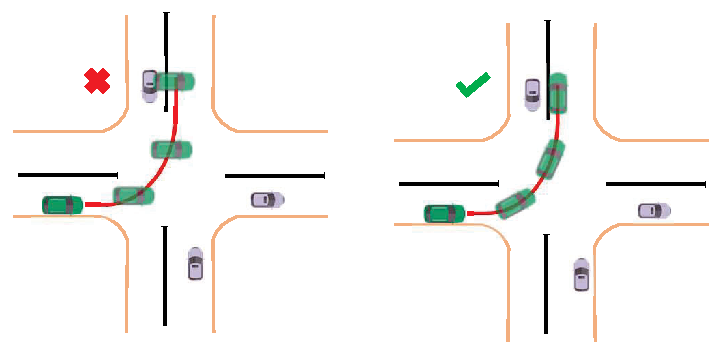
\includegraphics[width=1\linewidth]{Figures/Collision_Metric-Figure}
  \caption{}
  \label{fig:coll-rot}
  \end{subfigure}
    \begin{subfigure}{0.3\linewidth}
  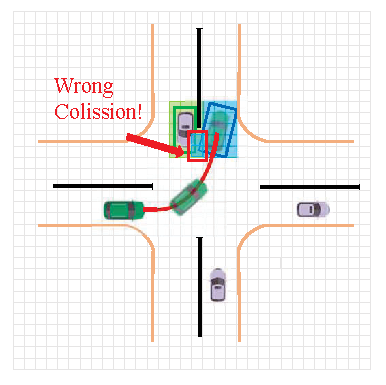
\includegraphics[width=1\linewidth]{Figures/Collision_Grid-Figure}
  \caption{}
  \label{fig:coll-grid}
  \end{subfigure}
  \caption{传统碰撞率计算方法的缺陷示意图。(a) 忽略自车偏航角变化可能导致错误的碰撞判断。(b) 占用网格的分辨率有限也可能导致错误的碰撞判断。}
  \label{fig:collision-metric}
\end{figure}
碰撞率是评估端到端自动驾驶方法中规划轨迹安全性的关键指标。然而，本文认为常用的碰撞率计算方法 \cite{hu2022st} 存在\textbf{两个显著缺陷}，导致评估结果不可靠。\textbf{首先}，正如先前研究所强调的\cite{li2023ego}，传统指标未考虑自车车头朝向的变化，特别是在转弯场景中，车辆的边界框方向不正确地保持为直行状态。在 \cref{fig:coll-rot} 中展示了此类情况。\textbf{其次}，先前研究常用的占用网格（OCC, Occupancy Grid）评估方法在效率和精度之间权衡，仅提供约0.5米的网格分辨率。然而，这种精度降低可能导致在评估中对自车与周围智能体之间发生碰撞的误判，因为在复杂场景中0.5米远大于自车与其他智能体之间可能的最小安全距离，这同样可能导致不可靠的评估，如 \cref{fig:coll-grid} 所示。

由于IMU可能存在的精度问题，自车的位置可能与其实际位置存在微小偏差，从而与驾驶场景中的其他智能体发生"碰撞"。在以往的碰撞率计算中，为确保自车真实轨迹无碰撞，真实轨迹的"碰撞"案例被排除在基准测试之外，不参与评估。然而，本文发现由于占用网格分辨率不足以及忽略自车偏航角变化，真实轨迹的"碰撞"情况被显著高估。如 \cref{tab:gt-collision} 所示，自车真实轨迹的"碰撞"率超过 \textbf{10\%}，即使考虑IMU误差，这在真实数据采集过程中也是\textbf{不可能}且\textbf{不可接受}的。

实际上，本文认为大多数误判的"碰撞"案例属于\textbf{困难案例（Hard Case）}，这是对规划进行全面评估的关键。不幸的是，这些困难案例被以往端到端自动驾驶方法中的规划性能评估排除了。为解决此问题，提出一种基于稀疏的方法来计算真实且精确的碰撞状态，用于端到端自动驾驶方法规划能力的可靠评估。具体而言，在计算每帧碰撞时，障碍物的位置及其车头朝向来自nuScenes数据集，自车的车头朝向通过比较规划轨迹中当前帧与前一帧的位置来近似。该方法消除了对占用网格的依赖，仅在自车边界框与其他障碍物边界框发生重叠时计算碰撞率。

如 \cref{tab:gt-collision} 所示，采用所提出的度量标准计算后，自车真实轨迹的碰撞率仅为 \textbf{0.58\%}，这更为合理，比粗粒度占用网格计算的结果低近20倍。\cref{fig:coll-rot} 展示了所提出的基于稀疏方法与传统的基于占用方法之间的差异。

出于与当前最优端到端方法进行公平比较以及充分验证所提出的基于稀疏的碰撞度量有效性的考虑，在所提出的度量标准下重新评估UniAD，并与SparseAD-B进行比较，如 \cref{tab:pred-collision} 所示。结果显示，UniAD\cite{hu2023planning} 的碰撞率相比其论文中的结果显著下降，这是由于引入了困难案例，这符合预期。

希望本节讨论及所提出的基于稀疏的碰撞度量能够启发和帮助端到端自动驾驶方法的未来研究。
